\chapter{Appendix: PREGO}

\section{Mappings}
\label{app:A}


PREGO produces entity identifiers either by Named Entity Recognition (NER) with the EXTRACT tagger or by mapping retrieved identifiers to the selected ones. 
PREGO adopted NCBI taxonomy identifiers for taxa, Environmental Ontology for environments and Gene Ontology as a structure knowledge scheme for Processes (GObp) and Molecular Functions (GOmfs). 
The latter was for reasons that are two-fold, first Gene Ontology has a Creative Commons Attribution 4.0 License and second there are many resources that have mapped their identifiers to Gene Ontology.
MG-RAST metagenomes and JGI/IMG isolates annotations come with KEGG orthology (KO) terms; 
Struo-oriented genome annotations, on the other hand, have Uniprot50 ids. 
The mapping from KO to GOmf and Uniprot50 to GOmf is implemented via UniProtKB mapping files of their FTP server (see \texttt{idmapping.dat} and \texttt{idmapping\_selected.tab} files). 
By using the 3-column mapping file, the initial annotations were mapped to GOmf. As a complement, a list of metabolism-oriented KEGG ORTHOLOGY (KO) terms has been built (see \textit{prego\_mappings} in the Availability of Supporting Source Codes section).
Finally, as STRUO annotations refer to GTDB genomes, \href{http://ftp.tue.mpg.de/ebio/projects/struo/GTDB_release89/metadata/}{publicly available mappings} (accessed on 24 December 2021) were used to link the genomes used with their corresponding NCBI Taxonomy entries.



\section{Daemons}
\label{app:B}

An important component PREGO approach (Figure A1) is the regular updates which keep PREGO in line with the literature and microbiology data advances. 
The updates are implemented with custom scripts called daemons that are executed regularly spanning from once a month up to six-month cycles. 
This variation occurs because of the API requirements of each web resource as well as the computational intensity of the association extraction from the retrieved data.

\begin{figure}[ht]
   \centering
   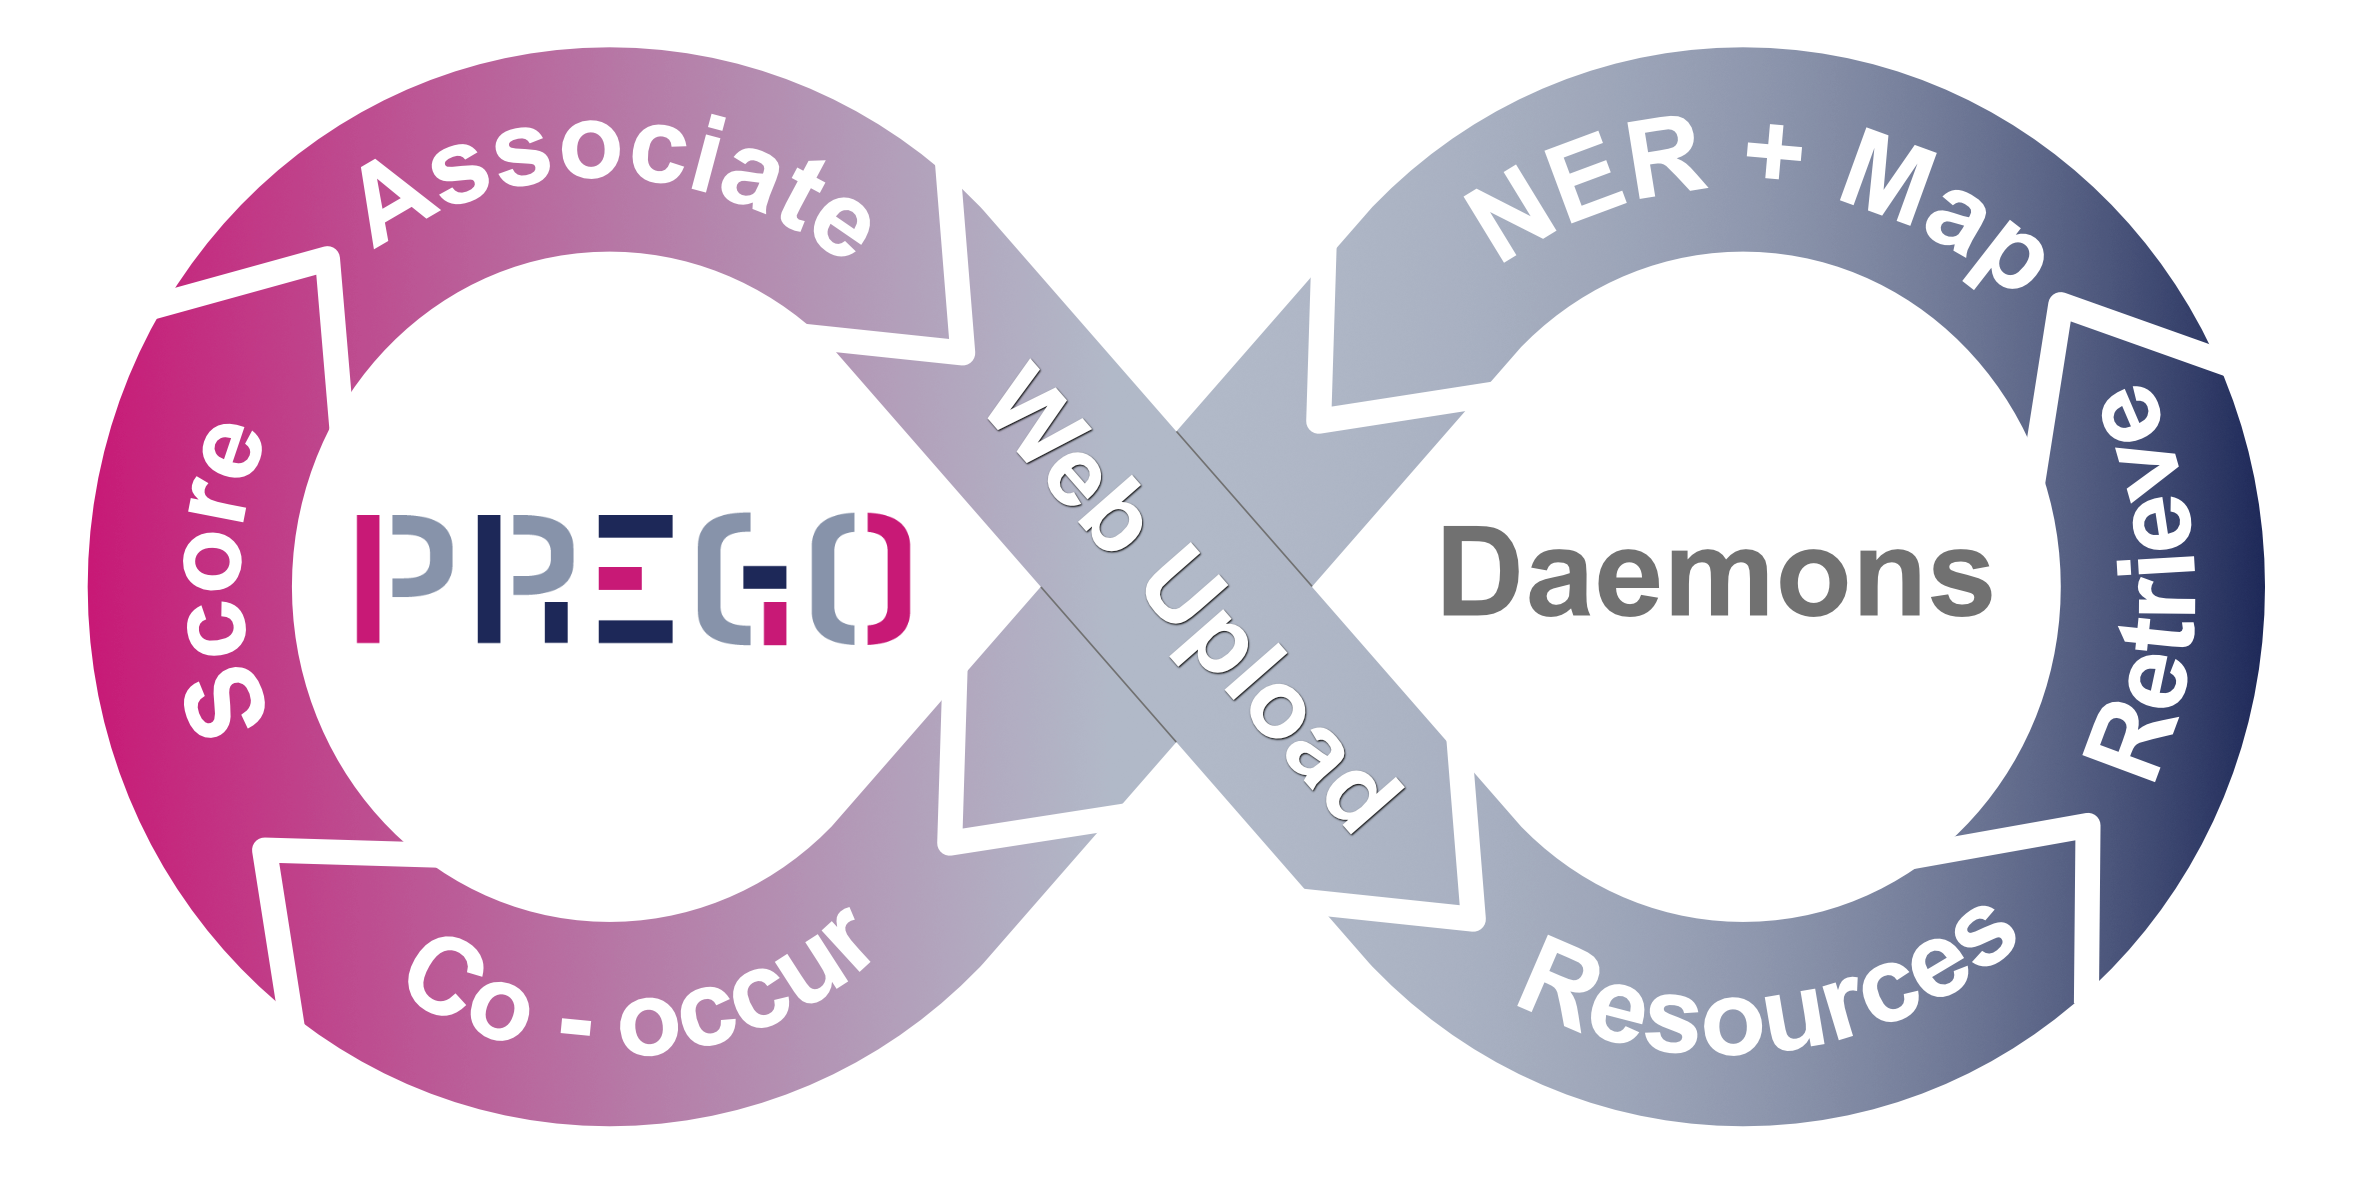
\includegraphics[width=95mm]{figures/figure_A1_PREGO_daemons.png}
   \caption[PREGO DevOps]{Software daemons perform all steps of the PREGO methodology in a continuous manner similar to the Continuous Development and Continuous Integration method.}
   \label{fig:devops}
\end{figure}


Each Daemon is attached to a resource because its data retrieval methods (API, FTP) and following steps, shown in Figure A1, require special handling and multiple scripts (see \textit{prego\_daemons} in the Availability of Supporting Source Codes section).

\section{Scoring}
\label{app:C}


Scoring in PREGO is used to answer the questions:
\begin{itemize}
   \item Which associations are more thrustworthy?
   \item Which associations are more relevant to the user's query?
\end{itemize}

Relevant, informative, and probable associations are presented to the user through the three channels that were discussed previously. 
Each channel has its own scoring scheme for the associations it contains and all of them are fit in the interval $(0,5]$ to maintain consistency. 
The values of the score are visually shown as stars. 
The Genome Annotation and Isolates channel has fixed values of scores depending on the resource because Genome Annotation is straightforward, and the microbe id is known a priori. 
On the other hand, Environmental Samples channel data are based on samples, which contain metagenomes and OTU tables. 
Thus, it has two levels of organization, microbes with metadata, and sample identifiers. Each association of two entities is scored based on the number of samples they co-occur. 
A Literature channel scoring scheme is based on the co-mention of a pair of entities in each document, paragraph, and sentence. The differences in the nature of data require different scoring schemes in these channels.
The contingency table (Table~\ref{table:pregoA1}) of two random variables, $X$ and $Y$ are the starting point for the calculation of scores. The term $X = 1$ might be a specific NCBI id and $Y = 1$ a ENVO term. 
The $c_{1,1}$ is the number of instances that two terms of $X = 1$ and $Y = 1$ are co-occurring, i.e., the joint frequency. 
The marginals are the $c_{1,.}$ and $c{.,1}$ for $x$ and $y$, respectively, which are the backgrounds for each entity type. 
Different handling of these frequencies leads to different measures. 
There is not a perfect scoring scheme, just the one that works best on a particular instance. 
Consequently, scoring attributes require testing different measures and their parameters.



\begin{table}[ht]
   \centering
   \begin{tabular}{c|llll}
    & \multicolumn{4}{l}{Y = y} \\ \cline{2-5} 
   \multirow{4}{*}{X = x} &  & Yes & No & Total \\ \cline{3-5} 
    & \multicolumn{1}{l|}{Yes} & $c_{x,y}$ & $c_{x,0}$ & $c_{x,.}$ \\
    & \multicolumn{1}{l|}{No} & $c_{0,y}$ & $c_{0,0}$ & $c_{0,.}$ \\
    & \multicolumn{1}{l|}{Total} & $c_{.,y}$ & $c_{.,0}$ & $c_{.,.}$
   \end{tabular}
   \caption[PREGO contingency table between two terms]{Contingency table of co-occurrences between entities $X = x$ and $Y = y$. 
   This is the basic structure for all scoring schemes. $c_{x,y}$ is the count of the co-occurrence of these entities. $c_{x,.}$ is the count of the $x$ with all the entities of $Y$ type (e.g., Molecular function). Conversely, $c_{.,y}$ is the count of $y$ with all the entities of $X$ type (e.g., taxonomy}
   \label{table:pregoA1}
\end{table}


\section*{Literature Channel}

Scoring in the Literature channel is implemented as in STRING 9.1 \citep{franceschini2012string} and COMPARTMENTS \citep{binder2014compartments}, where the text mining method uses a three-step scoring scheme. 
First, for each co-mention/co-occurrence between entities (e.g., Methanosarcina mazei with Sulfur carrier activity), a weighted count is calculated because of the complexity of the text.  


\begin{equation}
   c_{x,y} = \sum_{k=1}^{n}{w_d \delta_{dk}(x,y) +w_p \delta_{p,k}(x,y) + w_s \delta_{sk}(x,y)}
   \label{eq:prego-score-1}
\end{equation}



Different weights are used for each part of the document ($k$) for which both entities have been co-mentioned, $w_d = 1$ for the weight for the whole document level, $w_p = 2$ for the weight of the paragraph level, and $w_s = 0.2$ for the same sentence weight. 
Additionally, the delta functions are one (Equation~\ref{eq:prego-score-1}) in cases the co-mention exists, zero otherwise. Thus, the weighted count becomes higher as the entities are mentioned in the same paragraph and even higher when in the same sentence.
Subsequently, the co-occurrence score is calculated as follows:

\begin{equation}
   score_{x,y} = c_{x,y}^a (\frac{c_{x,y} c_{.,.}}{c_{x, .}c_{.,y}})^{1-a}
   \label{eq:prego-score-2}
\end{equation}
   


where $a = 0.6$ is a weighting factor, and the $c_{x,.}$, $c_{.,.}$, 
$c_{.,y}$ are the weighted counts as shown in Table~\ref{table:pregoA1} estimated using the same Equation~\ref{eq:prego-score-2}. 
This value of the weighting factor has been chosen because it has been optimized and benchmarked in various applications of text mining [34,70,71]. 
The value of Equation~\ref{eq:prego-score-2} is sensitive to the increasing size of the number of documents (MEDLINE PubMed—PMC OA).
Therefore, to obtain a more robust measure, the value of the score is transformed to $z$-score. 
This transformation is elaborated in detail in the COMPARTMENTS resource \citep{binder2014compartments}. 
Finally, the confidence score is the $z$-score divided by two. Cases in which the scores exceed the (0,4] interval are capped to a maximum of 4 to reflect the uncertainty of the text mining pipeline.

\section*{Environmental Samples Channel}

Data from environmental samples are OTU tables and metagenomes. Thus, for each entity x, the number of samples is calculated as the background and a number of samples of the associated entity (metadata background) c.,y (see Table A1). Each association between entities x, y has a number of samples, cx,y that they co-occur. Note that each resource is independent and the scoring scheme is applied to its entities. This means that the same association can appear in multiple resources with different scores. The score is calculated with the following formula:

\begin{equation}
   score_{x,y} = 2.0*\sqrt{\frac{c_{x,y}}{c_{.,y}}}^{ \:a}
\end{equation}


This score is asymmetric because the denominator is the marginal of the associated entity. 
Thus, the score decreases as the marginal of $y$ is increasing, i.e., the number of samples that $y$ is found. 
On the other hand, it promotes associations in which the number of samples of the association are similar to the marginal of $y$. 
The exponents on the numerator and denominator equal to $0.5$ and 
to $0.1$, respectively, in order to reduce the rapid increase of score.
Lastly, the value of the score is capped in the range $(0,4]$.


\section{Bulk download}
\label{app:D}

Users can also download programmatically all associations per channel through the links that are shown in Table~\ref{table:prego-appD-1}. 
The data are compressed to reduce the download size and md5sum files are provided as well for a sanity check of each download.

% PREGO BULK DOWNLOAD TABLE 
\begin{table}[ht]
   
   \begin{adjustwidth}{-1cm}{}

   \begin{tabular}{llll}
   \toprule
   Channel & Link & md5sum & Size (in GB) \\ \midrule

   Literature & \href{https://prego.hcmr.gr/download/literature.tar.gz}{literature.tar.gz} & \href{https://prego.hcmr.gr/download/literature.tar.gz.md5}{literature.tar.gz.md5} & 5.4 \\

   \begin{tabular}[c]{@{}l@{}}Environmental \\ Samples\end{tabular} &
   \href{https://prego.hcmr.gr/download/environmental\_samples.tar.gz}{environmental\_samples.tar.gz} & 
   \href{https://prego.hcmr.gr/download/environmental\_samples.tar.gz.md5}{environmental\_samples.tar.gz.md5}
   & 0.69 \\

   \begin{tabular}[c]{@{}l@{}}Annotated \\ genomes and \\ isolates\end{tabular} & 
   \href{https://prego.hcmr.gr/download/annotated\_genomes\_isolates.tar.gz}{annotated\_genomes\_isolates.tar.gz} &
   \href{https://prego.hcmr.gr/download/annotated\_genomes\_isolates.tar.gz.md5}{annotated\_genomes\_isolates.tar.gz.md5} & 0.26 \\ \bottomrule
   \end{tabular}
   \end{adjustwidth}
   \caption[PREGO Bulk download links and md5sum files.]{Bulk download links and md5sum files.}
   \label{table:prego-appD-comparisons}
\end{table}